\documentclass[11pt,a4paper]{article}

\usepackage[margin=1in]{geometry}
\usepackage[T1]{fontenc}
\usepackage[utf8]{inputenc}
\usepackage{setspace}
\usepackage{hyperref}
\usepackage{booktabs}
\usepackage{array}
\usepackage{longtable}
\usepackage{enumitem}
\usepackage{graphicx}
\usepackage{float}
\usepackage{amsmath}
\usepackage{amssymb}
\usepackage{caption}

\hypersetup{
  colorlinks=true,
  linkcolor=black,
  urlcolor=blue,
  citecolor=black
}

\setstretch{1.15}
\setlength{\parskip}{0.4em}
\setlength{\parindent}{0pt}

\title{\textbf{DSAI5201 Course Project Report (Option 2)}\\
Building a Lightweight RAG System for Academic Papers}

\author{
SHI Zhan (ID: 25043178g) \and
LUO Jiajie (ID: 25056154g) \and
FEI Yang (ID: 25042616g) \and
LI Weixin (ID: 25055774g)
}
\date{Spring 2026}

\begin{document}
\maketitle

\begin{abstract}
This report presents a lightweight Retrieval-Augmented Generation (RAG) system for academic papers.
The system builds a local vector database from paper files and answers user questions with retrieved context.
Our implementation integrates document parsing, chunking, embedding, vector retrieval, and large language model generation in a complete end-to-end pipeline.
We also provide reproducible code, demo results, and analysis of limitations.
\end{abstract}

\section{Project Scope and Motivation}
\textbf{Problem.}
Many students need to quickly understand multiple research papers, but manually searching long PDFs is time-consuming.

\textbf{Goal.}
Build a lightweight local RAG system that can answer questions based on academic paper content.

\textbf{Course alignment.}
This project follows Option 2 (Algorithm Implementation) and Category 3.1 (Building a Lightweight RAG System for Academic Papers).

\section{Technical Pipeline}
\subsection{System Overview}
The pipeline includes:
\begin{enumerate}[leftmargin=1.4em]
  \item document loading from local files,
  \item text cleaning and chunking,
  \item embedding and vector storage,
  \item retrieval with top-$k$ similarity search,
  \item answer generation with LLM using retrieved context,
  \item web-based demo for interactive QA.
\end{enumerate}

\subsection{Implementation Details (Based on Our Code)}
\textbf{Data ingestion.}
The index script auto-scans the \texttt{knowledge\_base/} folder and loads all supported formats (\texttt{.pdf}, \texttt{.md}, \texttt{.txt}, \texttt{.docx}).

\textbf{Parsing and chunking.}
PDF files are parsed by \texttt{UnstructuredPDFLoader} (high-resolution mode), then split by \texttt{RecursiveCharacterTextSplitter} with:
\begin{itemize}[leftmargin=1.4em]
  \item chunk size = 500
  \item chunk overlap = 50
\end{itemize}

\textbf{Embedding and vector DB.}
We use \texttt{bge-base-zh-v1.5} for embeddings and Chroma for persistent local vector storage.

\textbf{Retrieval and generation.}
We use query rephrasing + similarity retrieval from Chroma and send context + user query to Tongyi (\texttt{qwen-turbo}) to produce final answers.

\textbf{Demo interface.}
FastAPI + simple web front-end supports streaming answer display.

\section{Dataset and Experimental Setup}
\subsection{Paper Collection}
We use four academic papers placed in \texttt{knowledge\_base/}:
\begin{itemize}[leftmargin=1.4em]
  \item \texttt{Dynamic\_Graph\_Representation\_Learning\_for\_Spatio-Temporal\_Neuroimaging\_Analysis.pdf}
  \item \texttt{Federated\_Multi-Task\_Learning\_for\_Joint\_Diagnosis\_of\_Multiple\_Mental\_Disorders\_on\_MRI\_Scans.pdf}
  \item \texttt{Heterogeneous\_Structured\_Federated\_Learning\_with\_Graph\_Convolutional\_Aggregation\_for\_MRI-Based\_Mental\_Disorder\_Diagnosis.pdf}
  \item \texttt{SpatialTemporal\_Co-Attention\_Learning\_for\_Diagnosis\_of\_Mental\_Disorders\_From\_Resting-State\_fMRI\_Data.pdf}
\end{itemize}

\subsection{Environment}
\begin{itemize}[leftmargin=1.4em]
  \item Language: Python
  \item Core frameworks: LangChain, Chroma, FastAPI
  \item Embedding model: \texttt{bge-base-zh-v1.5}
  \item LLM API: Tongyi \texttt{qwen-turbo}
\end{itemize}

\subsection{Reproducibility}
We provide:
\begin{itemize}[leftmargin=1.4em]
  \item \texttt{requirements.txt}
  \item \texttt{README.md} with setup, indexing, and run instructions
  \item code repository link and demo steps
\end{itemize}

\section{Results and Demo Evidence}
\subsection{Functional Results}
The system successfully:
\begin{itemize}[leftmargin=1.4em]
  \item indexes local papers into vector database,
  \item retrieves relevant chunks for user questions,
  \item generates context-grounded answers in a web interface.
\end{itemize}

\subsection{Demo Cases}
\textbf{Case 1.} ``How is the SpatialTemporal Co-Attention mechanism constructed?''
The system returns a grounded explanation centered on the GCA-based co-attention design.

\textbf{Case 2.} ``Which paper uses federated learning, and what benefit does it claim?''
The system identifies federated-learning-related content and explains the privacy/generalization motivation.

\textbf{Case 3.} ``If we have small-sample MRI data, which method is more suitable and why?''
The system provides an application-oriented recommendation with supporting rationale from retrieved context.

\subsection{Demo Screenshots}
\begin{figure}[H]
  \centering
  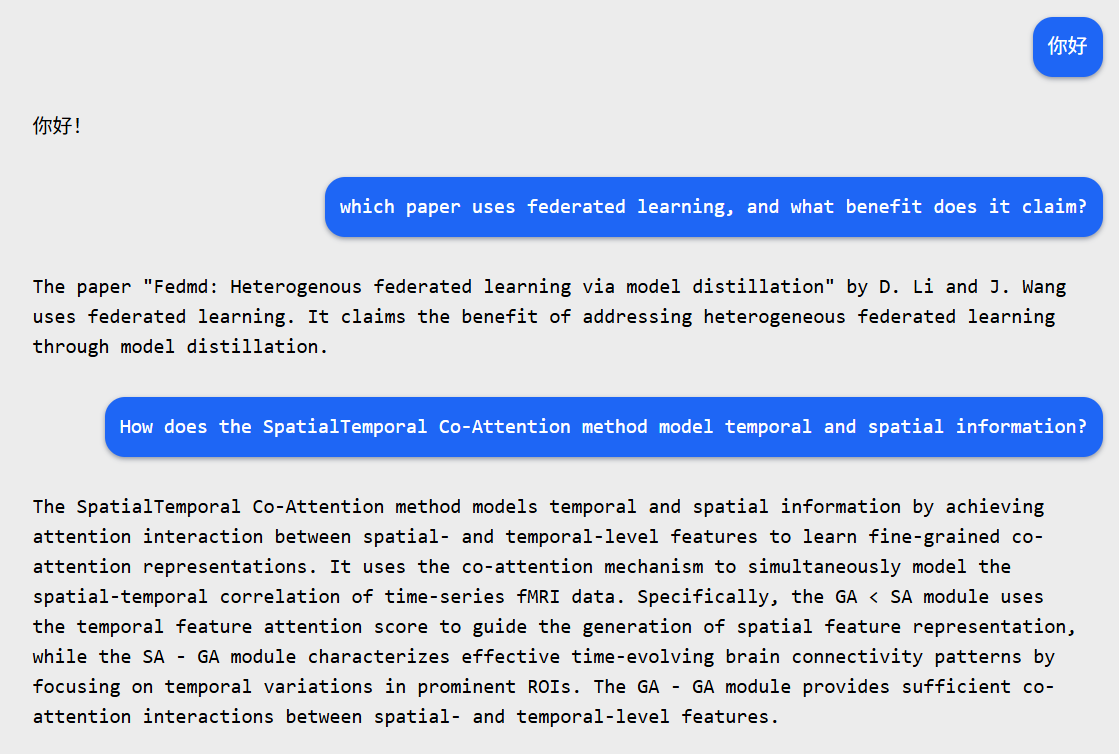
\includegraphics[width=0.92\textwidth]{../figs/1.png}
  \caption{Demo QA screenshot 1: responses for federated-learning and spatio-temporal modeling questions.}
  \label{fig:demo1}
\end{figure}

\begin{figure}[H]
  \centering
  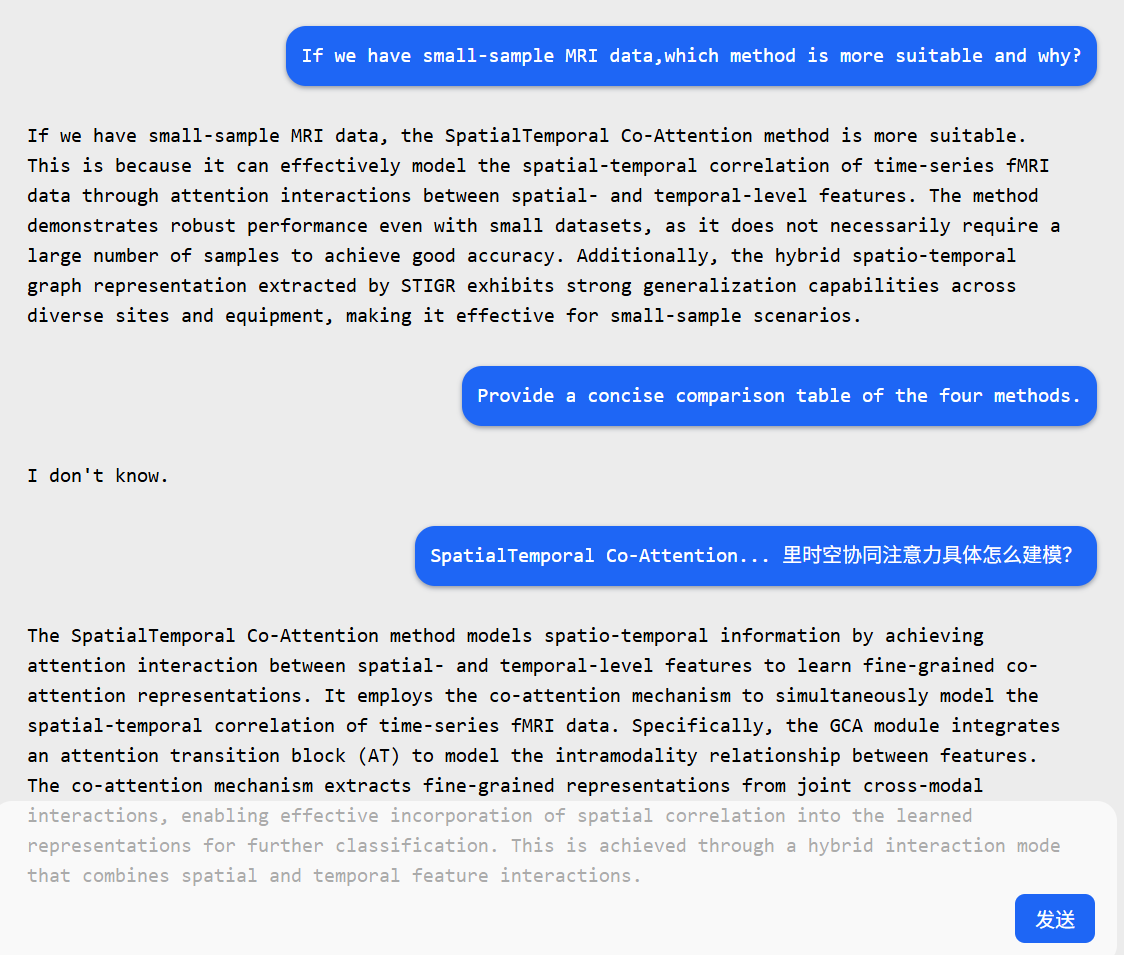
\includegraphics[width=0.92\textwidth]{../figs/2.png}
  \caption{Demo QA screenshot 2: response for the small-sample MRI scenario and follow-up explanation.}
  \label{fig:demo2}
\end{figure}

\section{New Contributions and Insights}
\textbf{Important note:} Running public code alone is insufficient for Option 2.
This section explicitly states our added contribution.

\begin{enumerate}[leftmargin=1.4em]
  \item \textbf{From fixed sample to scalable ingestion:}
  upgraded indexing from fixed sample files to automatic folder-wide multi-file ingestion.
  \item \textbf{Reproducibility enhancement:}
  added dependency lock file and execution guide so teammates can reproduce with three commands.
  \item \textbf{Practical deployment insight:}
  completed an end-to-end local demo (indexing + retrieval + generation + streaming UI), and summarized operational bottlenecks.
\end{enumerate}

\section{Limitations and Future Work}
\textbf{Current limitations:}
\begin{itemize}[leftmargin=1.4em]
  \item limited number of papers and domains,
  \item no strict quantitative metric benchmark yet,
  \item dependency on external LLM API quality and latency.
\end{itemize}

\textbf{Future work:}
\begin{itemize}[leftmargin=1.4em]
  \item increase paper coverage and create evaluation question set,
  \item add citation grounding and source highlighting,
  \item compare different embedding models and retrievers.
\end{itemize}

\section{Code and Demo Links}
\textbf{GitHub repository:} \url{https://github.com/leanderfei/5201RAG}

\textbf{Demo procedure:}
\begin{enumerate}[leftmargin=1.4em]
  \item \texttt{pip install -r requirements.txt}
  \item \texttt{python indexing.py}
  \item \texttt{python app.py}
  \item Open \url{http://127.0.0.1:8089} for QA demo
\end{enumerate}

\section*{References}
\begin{enumerate}[leftmargin=1.4em]
  \item Patrick Lewis, Ethan Perez, Aleksandra Piktus, et al. (2020). \textit{Retrieval-Augmented Generation for Knowledge-Intensive NLP Tasks}. arXiv:2005.11401. Available: \url{https://arxiv.org/abs/2005.11401}
  \item Rui Liu, Yao Hu, Jibin Wu, et al. (2025). \textit{Dynamic Graph Representation Learning for Spatio-Temporal Neuroimaging Analysis}. IEEE Transactions on Cybernetics, 55(3). DOI: \url{https://doi.org/10.1109/TCYB.2025.3531657}
  \item \textit{Federated Multi-Task Learning for Joint Diagnosis of Multiple Mental Disorders on MRI Scans}. (Paper used in local knowledge base, project dataset).
  \item \textit{Heterogeneous Structured Federated Learning with Graph Convolutional Aggregation for MRI-Based Mental Disorder Diagnosis}. (Paper used in local knowledge base, project dataset).
  \item \textit{SpatialTemporal Co-Attention Learning for Diagnosis of Mental Disorders From Resting-State fMRI Data}. (Paper used in local knowledge base, project dataset).
  \item LangChain Documentation. Available: \url{https://python.langchain.com/docs/introduction/}. Accessed: 2026-03-17.
  \item Chroma Documentation. Available: \url{https://docs.trychroma.com/}. Accessed: 2026-03-17.
  \item BAAI BGE Model Card (\texttt{bge-base-zh-v1.5}). Available: \url{https://huggingface.co/BAAI/bge-base-zh-v1.5}. Accessed: 2026-03-17.
  \item Tongyi Qwen API Documentation (DashScope). Available: \url{https://help.aliyun.com/zh/dashscope/}. Accessed: 2026-03-17.
\end{enumerate}

\newpage
\section*{Mandatory Statement of Contribution (One Full Page)}
\textbf{Course:} DSAI5201 AI and Big Data Computing in Practice \\
\textbf{Project Title:} Building a Lightweight RAG System for Academic Papers

\vspace{0.8em}

\vspace{1em}
\begin{longtable}{|p{0.22\textwidth}|p{0.33\textwidth}|p{0.37\textwidth}|}
\hline
\textbf{Name + Student ID} & \textbf{Responsible Sections} & \textbf{Task Description} \\
\hline
SHI Zhan (25043178g) &
Sections: \newline Technical Pipeline; Implementation Details; Retrieval and Generation &
Tasks: PDF parsing, text chunking, embedding model integration, vector database setup, retrieval module implementation, LLM invocation, RAG pipeline integration, and system testing. \\
\hline
LUO Jiajie (25056154g) &
Sections: \newline Dataset and Experimental Setup; Presentation Materials; Report Editing &
Tasks: academic paper collection, PPT production, and report writing/editing support. \\
\hline
FEI Yang (25042616g) &
Sections: \newline Technical Pipeline; Implementation Details; Results and Demo Evidence &
Tasks: PDF parsing, text chunking, embedding model integration, vector database setup, retrieval module implementation, LLM invocation, RAG workflow orchestration, and testing. \\
\hline
LI Weixin (25055774g) &
Sections: \newline Dataset and Experimental Setup; Presentation Materials; Report Editing &
Tasks: academic paper collection, PPT production, and report writing/editing support. \\
\hline
\end{longtable}

\vfill
\textbf{Group Declaration:}
We confirm that all members listed above contributed to this project, and section ownership has been clearly assigned for fair assessment.

\end{document}
